\documentclass{article}
\usepackage{parskip}
\usepackage[utf8]{inputenc}
\usepackage{mathptmx}
\usepackage{microtype}

\usepackage{graphicx}
\graphicspath{{images/}}
\usepackage{subcaption}
\usepackage{float}
\usepackage{amsmath}
\usepackage{multirow}
\usepackage{pdflscape}

\usepackage{listings}
\lstdefinestyle{withframe}{
  frame=single,
  showstringspaces=false, % don't mark spaces in strings
  commentstyle=\color{green}, % comment color
  keywordstyle=\color{blue}, % keyword color
  stringstyle=\color{red}, % string color
  basicstyle=\footnotesize\ttfamily,
}
\lstset{style=withframe}

\usepackage{cite}
\usepackage{color,soul}
\usepackage{hyperref}
\usepackage[toc,page]{appendix}

\title{CS5234 Project Report}

\author{
  Chan Wai Hap (A0178418U) \\
  \texttt{whchan@comp.nus.edu.sg}
  \and
  Lu Wei (A0040955E) \\
  \texttt{wei.lu@u.nus.edu}
}

\begin{document}

\maketitle

\tableofcontents

\pagebreak

\section{Overview}
The density of a graph is defined as the number of edges divided by the number of nodes.

\begin{equation}
  \rho(G) = \frac{m}{n}
\end{equation}

Where $m$ is the number of edges and $n$ is the number of nodes of graph $G$. This is a convention we are going to use consistently for the rest of this report.

A dense subgraph is induced by a set of nodes in the original graph with many edges connecting them. The problem of finding the densest subgraph for undirected graphs is first formalized by Andrew Goldberg in 1984 \cite{Goldberg:CSD-84-171}. He proposed a polynomial time exact algorithm for both unweighted and weighted graphs. It has been an active area research since. This class of problems are interesting not just from a theoretical perspective, they also have a lot of practical applications, such as community detection in social networks, web link spam detection for search engines, and correlation mining for gene, item or time series datasets. Such graph datasets are usually large with millions and even billions of nodes, which makes poly-time algorithm impractical. This prompts research in the direction of both distributed and approximation algorithms.

In our project, we limit the scope of our investigation to unweighted and undirect graphs. First, we explored both exact and approximation algorithms from existing literature for the densest subgraph problem, and formulated a distributed exact algorithm. For experimentation, we implemented Goldberg's exact algorithm, which we used to produce baselines for various datasets we experimented with. We then replicated and improved a MapReduce implementation of an approximation algorithm by Bahman et al in Hadoop – a distributed big data processing framework built on top of the MapReduce computational model. Last but not least, we also adopted the same approximation algorithm to a distributed graph processing framework named Giraph. We will present challenges and key lessons learned and compare the Hadoop and Giraph implementations.

\section{Algorithms and Theory}
In this section, we will introduce Goldberg's exact algorithm and briefly cover several approximation algorithms. Lastly, we will present our distributed exact algorithms and two possible realizations.

\subsection{Exact Algorithm}
The key idea of Goldberg's exact algorithm is to convert the original undirected, unweighted graph into a flow network as illustrated below:

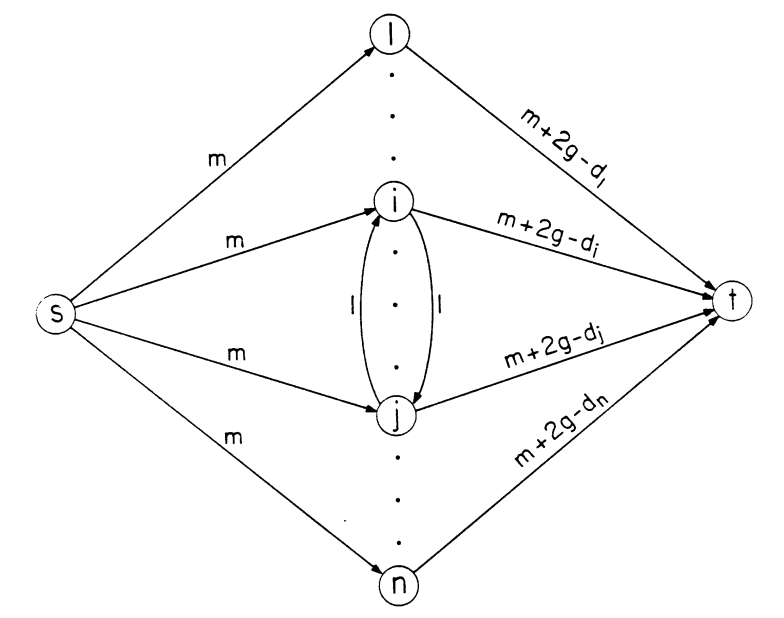
\includegraphics[width=\columnwidth]{goldberg_network.png}

Comparing to the original graph with nodes $V$ and edges $E$, the network has two nodes added: the source $s$ and the sink $t$: $V_N = V + \{s, t\}$, and $m + 2n$ edges added: $|E_N| = 2|E| + 2|N| = 2m + 2n$. Every original unweight and undirected edge is converted to two directed edges each with capacity 1. The capacity from $s$ to every node in the original graph is $m$; and the capacity from every node $i$ in the original graph to $t$ is assigned $m + 2g - d_i$, where $d_i$ is the degree of node $i$ in the original graph, and $g$ is a guessed value which the algorithm is going to iteratively ``sandwich'' by finding the min-cut until $g$ converges to the density of the densest subgraph.

The pseudocode for the algorithm is as below:

\begin{lstlisting}[mathescape=true]
  l=0, u=m, $V_1 = \emptyset$
  while $u - l > \frac{1}{n(n-1)}$ do
    $g = \frac{u+l}{2}$
    Construct network the updated g: $N = (V_N, E_N, g)$
    Find min-cut (S, T)
    if S = {s}
      u = g
    else
      l = g
      $V_1 = S - \{s\}$
  end
\end{lstlisting}

The intuition here is that the min-cut either goes throught all the out-edges of source node $s$, which looks like Case 1 below, or it doesn't (Case 2). In Case 1, the min-cut $c(S, T) = mn$; while for Case 2, the min-cut $c(S, T) = mn + 2n_1(g - \rho_1)$, where $n_1$ is the number of nodes in the subgraph induced by $V_1$ and $\rho_1$ is the density of the same subgraph. For detailed derivation please refer to the original paper \cite{Goldberg:CSD-84-171}. Notice that the $mn$ term appears in both cases, so for Case 2 to be the min-cut, it has to be the case that $2n_1(g - \rho_1) < 0 \Rightarrow g < \rho_1 \leq \rho^*$ where $\rho^*$ is the densest subgraph density. It follows that when Case 1 is the min-cut, $g > \rho^*$.

\begin{figure}[H]
  \centering
  \begin{subfigure}{.48\textwidth}
    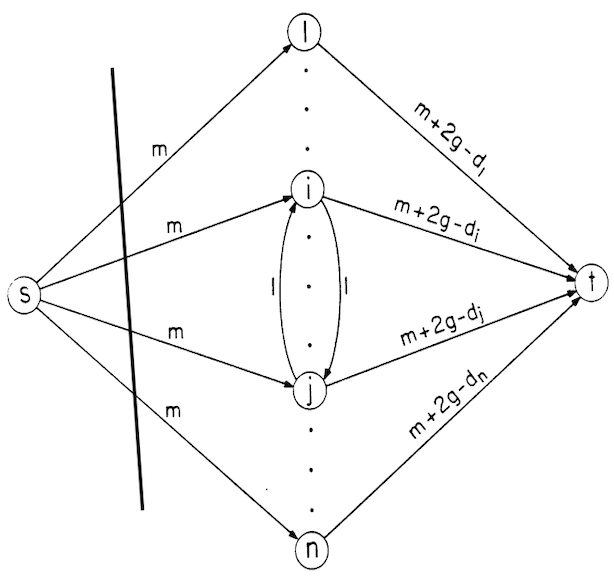
\includegraphics[width=\textwidth]{goldberg_network_cut1.png}
    \caption{Case 1}
  \end{subfigure}
  \begin{subfigure}{.48\textwidth}
    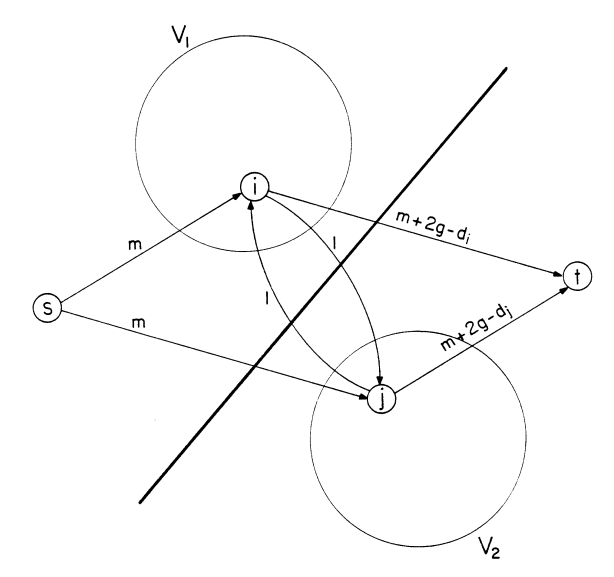
\includegraphics[width=\textwidth]{goldberg_network_cut2.png}
    \caption{Case 2}
  \end{subfigure}
\end{figure}

Since the value of $g$ is determined through binary search in the range of $[\frac{1}{n(n-1)}, m]$, it requires $log(n(n-1) \cdot m) = O(log(n^4)) = O(logn)$ iterations to terminate. Each iteration's running time is bounded by the time spent finding the min-cut in the contructed flow network.

There's extensive literature on finding s-t min-cut. The best known exact algorithm for general graphs is by Nagamochi and Ibaraki, which runs in time $O(mn + n^2logn)$ \cite{Nagamochi:1992:CEM:131829.131833}. In comparison, the classic push-relabel algorithm by Goldberg and Tarjan runs in $O(n^3)$ time for a sequential implementation \cite{Goldberg:1988:NAM:48014.61051}. Therefore for very dense subgraphs $m \approx n^2$, the best known min-cut algorithm's time complexity is also bounded by $O(n^3)$. Using $O(n^3)$ as the upper bound, the Goldberg densest subgraph algorithm described above has running time of $O(n^3logn)$.

We apprciate the cleverness of this algorithm in which one graph problem (densest subgraph) is translated to another graph problem (min-cut) through converting the original graph to a network flow with carefully assigned capacities. This is a common and effective technique we have come across while conducting literature review for this project.

\subsection{Approximation Algorithms}
We would like to focus on one approximation algorithm for finding densest subgraph in this section. It is proposed by Bahmani, Kumar, and Vassilvitskii \cite{Bahmani:2012:DSS:2140436.2140442}. The algorithm provides a $2 + 2\varepsilon$ approximation solution that completes in $O((m+n)logn$ time for a sequential implementation. We find this algorithm most impressive among its kind for the following reasons:

\begin{enumerate}
  \item Its distributed implementation completes in $O(logn)$ rounds,
  \item The algorithm itself is extremely simple, and
  \item It provides great close-to-truth approximation on real-world data.
\end{enumerate}

The key idea of this algorithm is to repeatedly remove small-degree nodes until the graph is empty. The intermediate subgraph with the highest density is the approximate solution to the densest subgraph problem. Below is the pseudocode:

\begin{lstlisting}[mathescape=true]
  $V_S, \tilde{V} = V$
  while $V_S \neq \emptyset$ do
    $V_R = \{i \in V_S | deg_S(i) \leq 2(1+\varepsilon)\rho_S\}$
    $V_S = V_S \ V_R$
    if $\tilde{\rho} < \rho_S$
      $\tilde{V} = V_S$
  end
\end{lstlisting}

Intuitively, this algorithm works because dense graph has large average degree, $\rho(G) = \frac{m}{n} = \frac{\sum_{i \in V}{deg_G(i)}}{2n} = \frac{1}{2} \textit{(average degree)}$. Therefore by removing small degree nodes, we expect the density of the subgraph induced by the remaining nodes to be large. The correctness and approximation bounds are established by setting the degree threshold carefully.

Let $V^*$ be the set of nodes in the true densest subgraph, $\rho^*$ be the true density. Removing any node i from $V^*$ will weakly reduce the density: $\rho^* \geq \rho(V^* \ \{i\}) = \frac{m^* - deg_{V^*}(i)}{n^* - 1}$. Since $n^* > 1$, we can multiply $n^* - 1$ on both sides of the inequality:

\begin{equation}
  \begin{split}
    \rho^* \cdot n^* - \rho^* & \geq m^* - deg_{V^*}(i) \\
    m^* - \rho^* & \geq m^* - deg_{V^*}(i) \\
    \rho^* & \leq deg_{V^*}(i)
  \end{split}
\end{equation}

Let i be a node in the true densest subgraph $ i \in V^*$, but we removed from $V_S$: $i \notin V_S$. This is bound to happen as $V_S$ is empty in the end. Since $V^* \subset V_S$ and i is removed because $deg_{V_S}(i) \leq 2(1+\varepsilon)\rho_S$. Combined with the inequality above, we have $\rho^* \leq deg_{V^*}(i) \leq deg_{V_S}(i) \leq 2(1+\varepsilon)\rho_S$, dividing $2(1+\varepsilon)$ on both sides:

\begin{equation}
  \rho_S \geq 2(1+\varepsilon) \rho^*
\end{equation}

This proves that the algorithm produces a $2(1+\varepsilon)$ approximation solution.

We can see that for every round of the algorithm, it reduces the graph size by a factor of at least $1+\varepsilon$. For node $i \in V_{St}$:

\begin{equation}
  \begin{split}
    \sum{deg_{V_{St}}(i)} & \geq n_{St} 2(1+\varepsilon)\rho_{S(t-1)} \\
    2 m_{S(t-1)} > \sum{deg_{V_{St}}(i)} & \geq n_{St} 2(1+\varepsilon) \frac{m_{S(t-1)}}{n_{S(t-1)}} \\
    \frac{n_{S(t-1)}}{n_{St}} & \geq (1+\varepsilon)
  \end{split}
\end{equation}

Therefore the algorithm terminates in $O(log_{(1+\varepsilon)}n)$ rounds. At each round, we check every node, which needs to count all its neighboring edges to get its degree, so the work per round is $O(m+n)$. Since degree is a node local property, the algorithm can therefore be distributed at every round.

\subsection{Distributed Exact Algorithms}
As a thought exercise, we explored possible formulations of a distributed exact algorithm for the densest subgraph problem. Our idea is to build the algorithm on top of Goldberg's min-cut based algorithm – we couldn't get around the outer loop which repeats $O(logn)$ times, so we looked into ways to distribute the min-cut finding algorithm, similar to how Bahmani's algorithm distributed the work within each round.

We came across a distributed min-cut algorithm by Nanongkai \& Su \cite{DBLP:journals/corr/NanongkaiS14}. They proposed a $1 \pm \varepsilon$ approximation algorithm based on finding a greedy tree packing: $(1 - \varepsilon) \rho^* \leq \rho \leq (1 + \varepsilon) \rho^*$. To obtain the exact min-cut, they proposed to first obtain a 3-approximation value $\rho'$ for the min-cut using another distributed algorithm by Ghaffari \& Kuhn \cite{DBLP:journals/corr/abs-1305-5520}, which guarantees that $\rho \leq \rho' \leq 3\rho^*$; then they set their error term $\varepsilon = 1/(\rho'+1)$ to obtain an exact solution:

\begin{equation}
  \begin{split}
      (1 - \varepsilon) \rho^* & \leq \rho \leq (1 + \varepsilon) \rho^* \\
      (1 - \frac{1}{\rho' + 1}) \rho^* & \leq \rho \leq (1 + \frac{1}{\rho' + 1}) \rho^* \\
      (1 - \frac{1}{\rho^* + 1}) \rho^* & \leq \rho \leq (1 + \frac{1}{\rho^* + 1}) \rho^* \\
      \rho^* - 1 & < \rho < \rho^* + 1 \\
      \rho & = \rho^*
  \end{split}
\end{equation}

The same paper claims that the algorithm runs in $O(\rho^{*4} log^2n (D + \sqrt{n} log^*n))$ rounds, where $D$ is the diameter of the graph. For detailed proof on the running time, please refer to the original paper.

Recall that for the converted network flow used in Goldberg's exact algorithm, $\rho^* = O(mn)$, therefore making the above time complexity $O(m^4 n^4 log^2n (D + \sqrt{n} log^*n))$ which is much worse than the time complexity for the sequential version of the original algorithm's $O(n^3logn)$, so it's impractical in our use case. Regardless, we still want to highlight the merit of Nanongkai's approach of using two approximation algorithms to arrive at an exact solution by setting appropriate value for the error term.

Next, we turned into the classic push-relabel algorithm by Goldberg \& Tarjan \cite{Goldberg:1988:NAM:48014.61051}. Turned out, this algorithm can be implemented in a distributed setting by breaking the push step into two substeps and perform the label update in between these two substeps. The pseudocode of the algorithm is presented as below. Note that a vertex v is active if it's label $0 < d(v) < n$ and it has excess flow: $e(v) > 0$.

\begin{lstlisting}[mathescape=true]
  For all active nodes v do
    <Push substep 1>
      push flow from v until flow excess $e(v) = 0$
        or there's no more residual capacity between v and
        any of its neighbor w: $d(w)=d(v)-1, r(v, w) = 0$
      reduce e(v) without increasing e(w)
    <Label update>
      if $e(v) > 0$
        $d'(v) = min(d(w) +1 | \forall w, r(v, w) > 0)$
        if $d(v) \neq d'(v)$
          $d(v) = d'(v)$
          send message $d(v)$ to all v's neighbors
    <Push substep 2>
      if there's any flow pushed to v in push substep 1
        increase e(v)
  end
\end{lstlisting}

The above procedure is repeated until there's no more active node. Since the described procedure only concerns node local properties and sending messages to the node's neighbors, it can be performed in parallel among all the active nodes.

The original paper stated and proved that the above procedure can be completed in $O(n^2)$ rounds, which makes our distributed exact algorithm for the densest subgraph problem run in $O(n^2logn)$ time. This is an improvement from the $O(n^3logn)$ time complexity of the original Goldberg min-cut based algorithm, however it's still $n^2$ factor slower than the $2+2\varepsilon$ approximation algorithm. This makes a good thought exercise, but this distributed exact algorithm is infeasible for large graphs with millions and billions of nodes.


\section{Implementations and experiments}
Among the algorithms described above, we've implemented Goldberg's min-cut based exact algorithmin python, and Bahmani's $(2+2\varepsilon)$ approximation algorithm in python, Hadoop and Giraph. In the following section, we will describe our implementations including the challenges we've faced and resolved and lessons learned.

\subsection{Baseline Implementation}
First, in order to provide the ground truth for any experiment datasets we may want to play with, we implemented Goldberg's exact algorithm. We chose to use the library graph-tool\footnote{Project homepage: \url{https://graph-tool.skewed.de/}} for this implementation for the following reasons:

\begin{enumerate}
  \item It provides an intuitive and effective python interface for handling graphs.
  \item Internally, its data structures and algorithms are implemented in C++, which makes it very fast. This makes it possible for us to play with bigger datasets, including graphs with tens of thousands of nodes.
  \item Conveniently, it comes with several min-cut algorithms\footnote{Available min-cut algorithm implementations: \url{https://graph-tool.skewed.de/static/doc/flow.html}} which we can use directly without having to implement it ourselves.
\end{enumerate}

Below is a sample output of our implementation executed on some of the Stanford Network Analysis Project (SNAP) graph datasets\footnote{SNAP datasets: \url{https://snap.stanford.edu/data/}}:

\footnotesize
\begin{lstlisting}[mathescape=true]
python densest_subgraph_goldberg.py
Processing data/ca-AstroPh_preprocessed.txt
original: # of nodes: 18772, # of edges: 198110, density: 10.5535
subgraph: # of nodes: 565, # of edges: 18147, density: 32.1186
function [process_graph] finished in 146275 ms

Processing data/ca-CondMat_preprocessed.txt
original: # of nodes: 23133, # of edges: 93497, density: 4.0417
subgraph: # of nodes: 30, # of edges: 404, density: 13.4667
function [process_graph] finished in 198157 ms

Processing data/ca-GrQc_preprocessed.txt
original: # of nodes: 5242, # of edges: 14496, density: 2.7654
subgraph: # of nodes: 46, # of edges: 1030, density: 22.3913
function [process_graph] finished in 11083 ms

Processing data/email-Enron_preprocessed.txt
original: # of nodes: 36692, # of edges: 183831, density: 5.0101
subgraph: # of nodes: 555, # of edges: 20726, density: 37.3441
function [process_graph] finished in 538753 ms

Processing data/ca-HepPh_preprocessed.txt
original: # of nodes: 12008, # of edges: 118521, density: 9.8702
subgraph: # of nodes: 239, # of edges: 28442, density: 119.0042
function [process_graph] finished in 71956 ms

Processing data/ca-HepTh_preprocessed.txt
original: # of nodes: 9877, # of edges: 25998, density: 2.6322
subgraph: # of nodes: 32, # of edges: 496, density: 15.5
function [process_graph] finished in 33418 ms
\end{lstlisting}

\normalsize

We preprocessed the edge list data from SNAP because we noticed that though the datasets are labelled ``undirected'', it's not always guaranteed that every node pair only appears once, nor the matching reverse pair always exists. Our preprocessing script scans through all the edges and if $(a, b)$ and $(b, a)$ both exist, we only keep one of them in the \texttt{*\_preprocessed.txt} files.

Running the exact algorithm implementation on real-world data provides us with the ground truth of the densest subgraphs. We used results from this exercies to verify that our Hadoop and Giraph implementations of the approximation algorithm produce correct results within the theoretical bounds. In addition, the timing information is also useful as performance baseline to gauge the scale of data a single machine is able to handle, for example, according to the above output, on a MacBook Air with 1.6 GHz Intel Core i5 processor, with 16 GB RAM, it took about 9 minutes to execute the exact algorithm on the Enron email dataset which has 36K+ nodes.

This exercise of implementing Goldberg's exact algorithm also helped us better understand the algorithm, which gave us the idea of formulating the distributed version of the algorithm described above.

\subsection{Hadoop Implementation \& Improvement}
Hadoop is an open source implementation of the MapReduce programming model proposed by Dean and Ghemawat from Google. The MapReduce model is designed to facilitate general purpose distributed big data processing \cite{Dean:2004:MSD:1251254.1251264}. A MapReduce job is made of two phases: the Map phase reads key-value pairs from a distributed file system and perform operations such as filtering and transformation and emit intermediate key-value pairs as output. The framework then takes care of shuffling the intermediate output and group them by key and send those with the same key to the same reducer for the Reduce phase. The Reduce phase is analogous to the reduce function in functinoal programming. This is where values of the same key can be aggregated or tallied according to the user defined reduce function. The output of the Reduce phase is then written into the distributed file system. Multiple MapReduce jobs can be chained to form a workflow to handle general purpose data processing at scale.

The MapReduce model heavily relies on the underlying distributed file system to efficiently manage data distribution and replication. One groundbreaking idea of MapReduce is to bring the computation to data whenever possible, rather than moving data from a separate storage to computation clusters. This in a distributed setting saves time spent on network IO which speeds up the data processing. Hadoop comes with its own implementation of the distributed file system named Hadoop Distributed File System (HDFS).

We used Hadoop Streaming with Python to implement the densest subgraph approximation algorithm. Hadoop Streaming is a Hadoop utility that enables creating and running MapReduce jobs with any executable or script as mappers/reducers. The scripts simply need to read the streaming input through \texttt{stdin}. This utility allows MapReduce jobs to be written in other programming languages besides the de facto framework language Java.

In order to process the graph data in a distributed fashion, we first uploaded the edge list data to HDFS. There are three essential MapReduce stages for our implementation: degree counting, threshold calculation, and node removal.

To count the degrees for each node of input graph, the mapper maps each undirected edge $(u,v)$ in the graph into two key-value pairs: $(u, v), (v, u)$; the reducer then simply counts the number of values for each key that represents the node id for each node. The reducer emits both the original node pairs as well as the tallied degrees formatted as $(u, "d", degree)$. Having two fields as value for the degree output allows us to identify and filter such key-value pairs in our subsequent MapReduce stages.

The threshold mapper reads the output from the previous MapReduce job and filter only the key-value pairs with degrees and emits $("n", 1)$ and $("2m", degree)$ for each key-value pair. The reducer then aggregates all the ``n'' values to get the total number of nodes, and ``2m'' values to obtain 2 times the total number of edges. It then calculate the density of the current graph and the degree threshold needed for node removal, and store the output on HDFS.

To perform node removal, we need to remove every edges in the graph that are associated to the nodes with degree below threshold during each iteration. It requires two MapReduce passes. For each edge pair $(u,v)$, the mapper first uses $u$ as the mapping key, and it emits an additinal special key-value pair $(u, \$)$ when the mapper reads a node degree below the threshold, otherwise it just copies the input key-value pair. When the reducer later receives input with values containing the special character \$, it omits all the values associated with that key, otherwise, it copies every key-value pair and emit them. In the second pass, the mapper then uses $v$ as the mapping key, and perform the same action; and so does the reducer.

\hl{TODO Xavier: add experiment results on actual improvement from merging degree counting \& node removal step.}
Our attempted improvement is that, for each iteration instead of running all these two stages as three different MapReduce phases, we have managed to combine the degree counting into the second phase of node removal, which significantly eliminates the overhead of running an extra MapReduce phase.

\subsection{Giraph Adaptation}
Giraph is an open source distributed data processing framework specifically designed for processing graphs. It implements the Pregel computational model \cite{Malewicz:2010:PSL:1807167.1807184}, which in turn is inspired by Valiant’s Bulk Synchronous Parallel model \cite{Valiant:1990:BMP:79173.79181}. It models the data processing as a sequence of iterations, each iteration is called a ``superste''. At each superstep, a user defined function is executed, conceptually in parallel for every node of the graph. A vertex can perform update and mutation actions such as changing its label data and removing its neighboring edges, as well as sending messages to its neighboring nodes over outgoing edges and processing any incoming messages from the previous superstep.

Giraph is built on top of Hadoop, since both distributed computational models let user focus on local actions and a superstep can naturally be translated to a MapReduce step. Giraph also added additional features beyond what is described in the original Pregel paper, such as master computation which can be used to facilitate global computation and coordination before the execution of the node centric user defined function of a superstep. This is particularly useful in our case as the algorithm requires calculating the density of the remaining graph at every iteration. During our implementation we find it conceptually helpful to think of a superstep as made of a \texttt{MasterCompute} substep followed by a \texttt{BasicCompute} substep.

To adapt the densest subgraph approximation algorithm to Giraph, first we need to duplicate and reverse the input edge list in order to represent undirect graphs. Giraph comes with a built-in java class \texttt{IntNullReverseTextEdgeInputFormat} which handles this exact case. Then we define our vertex centric function as part of the \texttt{BasicComputate} substep:

\begin{lstlisting}
  Get degree threshold value computed by MasterCompute
  If the node's degree (getNumEdges) is smaller than the threshold:
    Remove current node in the next superstep (removeVertexRequest)
    Message all neighbors to remove in-edges (sendMessageToAllEdges)
  For every message received from previous superstep:
    remove out-edge (removeEdges)
\end{lstlisting}

And for our \texttt{MasterCompute}:

\begin{lstlisting}
  If total number of nodes (getTotalNumVertices) is zero, terminate
  Calculate current density and degree threshold
  Update global Aggregator value for threshold
  Read maximum density from a global Aggregator
  If max density smaller than current density:
    update Aggregator max density to current density value
\end{lstlisting}

Communication between \texttt{MasterCompute} and \texttt{BasicCompute} is achieved through \texttt{Aggregators} which is initialized and registered by \texttt{MasterCompute} upon its own initialization. Internally, it reads and writes values onto the distributed file system (HDFS).

Note that every node owns its outgoing edges, but not its incoming edges. This means that removing a node also removes its outgoing edges, but not its incoming edges. Since each \texttt{BasicCompute} substep is node local, any attempt at removing an edge that a node doesn't own will not take any effect, including any of its incoming edges. Therefore we utilize messaging to signal the edge owner to remove the incoming edges of any removed node.

Giraph also keeps track of every node's degree and totally number of edges and nodes of the graph by default. However, it's worth pointing out that although total number of edges and nodes are accessible at any time for both \texttt{MasterCompute} and \texttt{BasicCompute}, the values are only consistent with the state of the graph from the previous superstep. In addition, not all mutation operations are executed instantly: In our case, \texttt{removeEdges} is considered a vertex-local operation so it's instantly executed in the same superstep, but \texttt{removeVertexRequest} is only carried out by the framework in the next superstep. Combining the lagged view and delayed operation, it means that the \texttt{MasterCompute} will only observe the updated total number of nodes and edges resulted from node removal 2 supersteps later; while \texttt{MasterCompute} will observe the updated total number of nodes and edges resulted from edge removal 1 supersteps later. This is important to note as it was a source of bug when synchronization is required to guarantee correctness of the algorithm. A common technique used is to check the current superstep count (\texttt{getSuperstep}), and perform different actions accordingly, e.g. only perform action 1 on even supersteps. Our adoption of the same technique resulted in the following Giraph workflow:

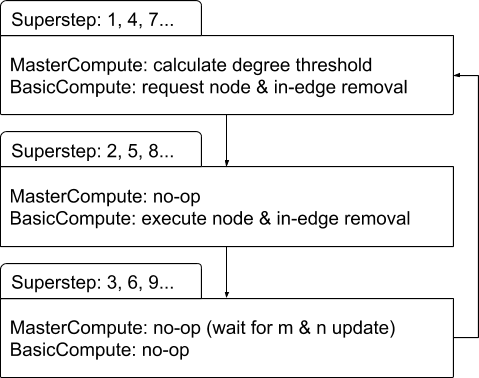
\includegraphics[width=0.8\columnwidth]{giraph_job.png}

Another caveat to note is that by default, Giraph will recreate a deleted node when any message is received by that node. This behavior can be disabled through job run configuration option \texttt{giraph.vertex.resolver.create.on.msgs}.

In the process of implementing the Giraph adaption of the approximation algorithm, we realized that it's difficult to reason and debug such a distributed program due to unfamiliarity with the framework. One thing that really helped speed up the debugging process is to implement the approximation algorithm in pure python and print out the expected number of nodes, edges and degree threshold at every iteration. Since the algorithm is simple and runs fast, the python implementation is quick to implement and easy to run on a small dataset. By comparing the debug output from the python program and the Giraph program, we are able to track down the sources of the issues and understand quirks and features of the Giraph framework.

\subsection{Experiment Results}
Below we present the densest subgraph density produced by our various implementations:

\begin{landscape}
\begin{tabular}{|c|c|ccc|ccc|ccc|}
\hline
                               & Python (exact) & \multicolumn{3}{|c|}{ Python (approximation) } & \multicolumn{3}{|c|}{ Hadoop } & \multicolumn{3}{|c|}{ Giraph }   \\
Dataset                        & Actual Density & $\varepsilon=0.001$ & $\varepsilon=0.1$ & $\varepsilon=1$ & $\varepsilon=0.001$ & $\varepsilon=0.1$ & $\varepsilon=1$ & $\varepsilon=0.001$ & $\varepsilon=0.1$ & $\varepsilon=1$ \\
\hline
\multirow{2}{*}{ ca-AstroPh }  & 32.119         & 28.018  & 27.971  & 26.359                   & 28.009  & 27.980  & 26.354   & 28.018  & 27.971  & 26.359     \\
                               & approx/actual  & 1.146   & 1.148   & 1.219                    & 1.147   & 1.148   & 1.219    & 1.146   & 1.148   & 1.219      \\
\hline
\multirow{2}{*}{ ca-CondMat }  & 13.467         & 12.615  & 12.615  & 8.726                    & 12.558  & 12.558  & 8.682    & 12.615  & 12.615  & 8.726      \\
                               & approx/actual  & 1.067   & 1.067   & 1.543                    & 1.072   & 1.072   & 1.551    & 1.067   & 1.067   & 1.543      \\
\hline
\multirow{2}{*}{ ca-GrQc }     & 22.391         & 22.391  & 21.956  & 18.209                   & 22.391  & 20.500  & 18.819   & 22.391  & 21.956  & 18.209     \\
                               & approx/actual  & 1.000   & 1.020   & 1.230                    & 1.000   & 1.092   & 1.190    & 1.000   & 1.020   & 1.230      \\
\hline
\multirow{2}{*}{ ca-HepPh }    & 119.004        & 119.004 & 117.926 & 117.697                  & 119.002 & 117.924 & 117.695  & 119.004 & 117.926 & 117.697    \\
                               & approx/actual  & 1.000   & 1.009   & 1.011                    & 1.000   & 1.009   & 1.011    & 1.000   & 1.009   & 1.011      \\
\hline
\multirow{2}{*}{ ca-HepTh }    & 15.500         & 15.500  & 15.500  & 8.286                    & 15.500  & 15.500  & 8.407    & 15.500  & 15.500  & 8.286      \\
                               & approx/actual  & 1.000   & 1.000   & 1.871                    & 1.000   & 1.000   & 1.844    & 1.000   & 1.000   & 1.871      \\
\hline
\multirow{2}{*}{ email-Enron } & 37.340         & 35.306  & 34.192  & 32.390                   & 35.306  & 34.192  & 32.390   & 35.306  & 34.192  & 32.390     \\
                               & approx/actual  & 1.058   & 1.092   & 1.153                    & 1.058   & 1.092   & 1.153    & 1.058   & 1.092   & 1.153      \\
\hline
\end{tabular}

As we can see, our approximation implementations produced consistent results and they are within the theoretical bounds when compared with the ground truth results.

\end{landscape}


\section{Conclusion}
In this project, we explored both exact and approximation algorithms for finding the densest subgraph for undirected and unweighted graphs. The key takeaways from the theory front are summarized as follow:

\begin{enumerate}
  \item We can convert a new graph problem to a different one to which there's already existing algorithms solutions. We've seen this done in Goldberg's exact algorithm for densest subgraph where he converted the graph to a network flow, and reduced the problem to finding minimum cut repeatedly.
  \item It's possible to convert some approximation algorithm to exact algorithm by setting appropriate values for the error term. We've seen this done by Nanongkai \& Su in their distributed approximation algorithm.
  \item A sequential algorithm can be converted to a distributed algorithm by distributing work within each iteration. We've done this as a thought exercise in formulating a distributed exact algorithm for finding densest subgraph based on Goldberg's algorithm.
\end{enumerate}

On the implementation and experiment front, we've successfully implemented Goldberg's exact algorithm and Bahmani's approximation algorithm in python. We've implemented and improved the Hadoop implementation of Bahmani's approximation algorithm using Hadoop Streaming. We also adapted the same algorithm to the Giraph framework. We presented the challenges we faced and resolved in the implementation process. Not only we've learned the quirks and features of distributed data processing frameworks Hadoop and Giraph, also we learned useful lessons on debugging distributed implementations:

\begin{enumerate}
  \item It's helpful to have a reference non-distributed implementation of an algorithm. This is especially useful when one is dealing with an unfamiliar distributed framework.
  \item To verify correctness, start with a small dataset on a single worker/node. This makes debugging easier to reason.
  \item Before setting up and experimenting on multiple remote instances, first make sure the program behaves correctly locally with multiple workers. This saves time and money.
\end{enumerate}

\newpage

\begin{appendices}
\section{Source Code}
All source code is available at \url{https://github.com/weilu/cs5234}. Please follow the setup instructions in the README.

\begin{itemize}
  \item Data folder: \href{https://github.com/weilu/cs5234/tree/master/data}{/data}
  \item Data preprocessing: \href{https://github.com/weilu/cs5234/blob/master/preprocess.py}{preprocess.py}
  \item Goldberg's exact algorithm: \href{https://github.com/weilu/cs5234/blob/master/densest_subgraph_goldberg.py}{densest\_subgraph\_goldberg.py}
  \item Bahmani's approximation algorithm (non-distributed): \href{https://github.com/weilu/cs5234/blob/master/densest_subgraph_approx.py}{densest\_subgraph\_approx.py}
  \item Bahmani's approximation algorithm Hadoop implementation: \href{https://github.com/weilu/cs5234/tree/master/hadoop}{/hadoop}
  \item Bahmani's approximation algorithm Giraph implementation: \href{https://github.com/weilu/cs5234/tree/master/giraph/}{/giraph}
  \item Bahmani's approximation algorithm Hadoop implementation executable on AWS EMR: \href{https://github.com/weilu/cs5234/tree/hadoop2/hadoop2}{folder /hadoop2 on git branch hadoop2}
\end{itemize}
\end{appendices}

\newpage

\bibliography{reference}{}
\bibliographystyle{plain}

\end{document}
